%This file should include Discussion, Future works and Conclusion
\chapter{Discussion}
When evaluating the data acquired during the earlier chapter, it is important to account for two things: validity and reliability. In this chapter we discuss the findings from our evaluation.
\section*{Validity}
	Validity is defined as:\\
	\begin{quote}
		\textit{Validity is concerned with whether the evaluation method measures what it is intended to measure}\cite{interactionDesign}.\\
	\end{quote}
	What this roughly means, is how much the data can be trusted, as in if the there can be potential variations that might invalidate the data. Some potential causes for and against the validity of our two tests could be:\\
	\begin{enumerate}
		\item The tests both took place in our group room, where there could have been noise, and distractions from outside people, that could have made the participants less focused on the test at hand.\\
		
		\item Most of, if not all, of the participants that were found utilizing convenience sampling, were students AAU CPH, and as such aren't very likely representative of how the actual target group would have behaved during the test.\\
		
		\item Due to the semi-structured nature of the immersion test, some participants might have been confused, and therefore not been able to focus completely on the test, but rather on talking with the moderator conducting the test, to make sense of it.\\
		
		\item Both tests had a small sample size, this might have resulted in certain trends not being discovered unless a bigger sample was introduced.\\
		
		\item During both tests we used the same laptop for running the VR unit, a laptop which is not powerful enough to run the virtual environment smoothly enough to be comfortable (See \autoref{fig:barChartFrame}).\\
		
		\item The participants in both tests, might have given more positive responses, simply due to the fact that most have not tried Virtual Reality before, and even if they had, it is very new and "\textit{cool}" technology that is exciting to play with.
		
	\end{enumerate}

\section*{Reliability}
	Reliability is defined as:\\
	\begin{quote}
		\textit{The reliability or consistency of a method is how well it produces the same results on separate occasions under the same circumstances}\cite{interactionDesign}.\\
	\end{quote}
	Which means how much you can rely on the tests producing the same results, under the same circumstances, if the test was run on separate occasions by other researchers. Some of the factors we considered relevant to reliability are:\\
	\begin{enumerate}
		\item For the usability test, we made a plan for how the test should be set up, as seen in \autoref{fig:test1}. This was to make it so that every instance of the test ran as close to identically as possible.\\
		
		\item For the immersion test, there's was no such plan, and due to the test being split up into 3 separate parts, it was semi-structured at best. Due to the semi-structured setup of the test, there were also no minimum or maximum time each participant spent on each part, they simply spent the time they each thought was adequate.\\
		
		\item The usability test followed a manuscript (See \autoref{sec:appendixUsabilityManuscript}), to make sure there was as little inconsistency as possible.\\
		
		\item The immersion test did not have any manuscript, but merely some rough and loose guidelines to follow; explaining about the three parts of the test, and that the participant should try to visualize being in the garden. This could potentially make it harder to replicate the test procedure.\\
	\end{enumerate}
	The tests have shown that the prototype might have some usefulness for people role playing as garden architects. The tests has proven the prototype as a proof of concept, wherein other researchers can continue development and study in the future.
	

\chapter{Conclusion}
We can therefore conclude that the prototype is indeed more immersive than traditional 2D sketching and 3D viewing of gardens. We can't, however, conclude if our prototype is better than conventional sketching methods, for conveying garden design ideas to customers.\\\\


In order to get a comfortable and aesthetically pleasing garden around the house, one could get in touch with a landscape architect, although if a simple 2D sketch is not a sufficient visualization of their design there are most likely going to be additional expenses involved, and possibly also a longer waiting period.

The landscape architects usually include their clients in the design process and therefore it would be relevant to consider these clients as a secondary target group. Based on the client related questions it is clear that the target groups primary customers range from around 25 to 60 years. There are no distinctive design elements that are heavily used. The trends are that the gardens should be maintenance-free and have plants that are able to survive the Danish climate due to shifting weather through the year. The architects customer can sometimes have a hard time understanding the three-dimensional space of their future garden when it is only presented on a sketch. Even though some landscape architects use 3D visualization it has to be an easy and efficient process in order to keep the cost down. Otherwise the customers will probably do without it.

Most of the questionnaire respondents were familiar with VR and felt comfortable using it. The group that expressed most comfort with it were aged 36-45, which is within the age group defined by the experts in section\autoref{sec:expertInterviews}
The garden sizes vary quite a bit although many of the respondents' gardens were larger than 800m² and the second largest group were in between 500-800m². This indicates that the ability to scale the garden would be useful. If the project ends up being limited in the number of models included, it would make sense to at least include the common garden plants shown in \autoref{fig:plantlist}.\\\\
\section*{FPS}
How can creating a 3D VR environment in a fast and efficient manner, using fiducial markers on a physical implementation, help garden architects give their customers more insight into what it would be like to be in the garden during their design process at the customers garden?


\chapter{Future Works}
Looking at our results from our previous tests, we now know what work has to be done on our prototype to improve it in the future. We got some feedback in regards to where the client was in the garden while the architect was building it on the glass plate. In addition to this some kind of marker could be installed to track where the client was in the VR world and that would show op on the glass plate for the architect to know exactly where the client was at that moment. To which degree how easy or difficult this would be to install is not considered yet, but it needs to be efficient and not slowing down the system or being more cumbersome than necessary.\\

Another way to ease our prototype is to make it lighter. Basically this would be using another more transportable VR unit, that doesn't need as much setup time as it do right now. Further more another webcam would be preferred.\\
Regarding the box, it needs to be the right size for the camera used so that we don't have any parts on the glass plate where the marker wont show up in the VR world. The box itself would be made lighter and in a way that makes it easier to transport.\\

\textbf{Allow architects to draw sections on the plate, then place a marker inside them to place multiple objects, or change texture}. One problem with the current implementation is that it is impossible to do things like a flowerbed. During the usability test one test person also remarked that the ability to create custom shaped pond would be nice. The idea is reasonably simple, one can draw enclosed shapes on the plate. Placing a marker inside this will cause the entire shape to be filled with the marker's object. Rotating the flower would control the density of the objects in the shape. This could also be used to add things like tiled paths, or walls to the garden, making it look way more like a real garden. How the implementation could work can be seen in Figure \ref{fig:ftemarkers}, and \ref{fig:ftrmarkerslegend}.
\begin{figure}[H]
	\centering
	\begin{minipage}[b]{0.49\textwidth}
		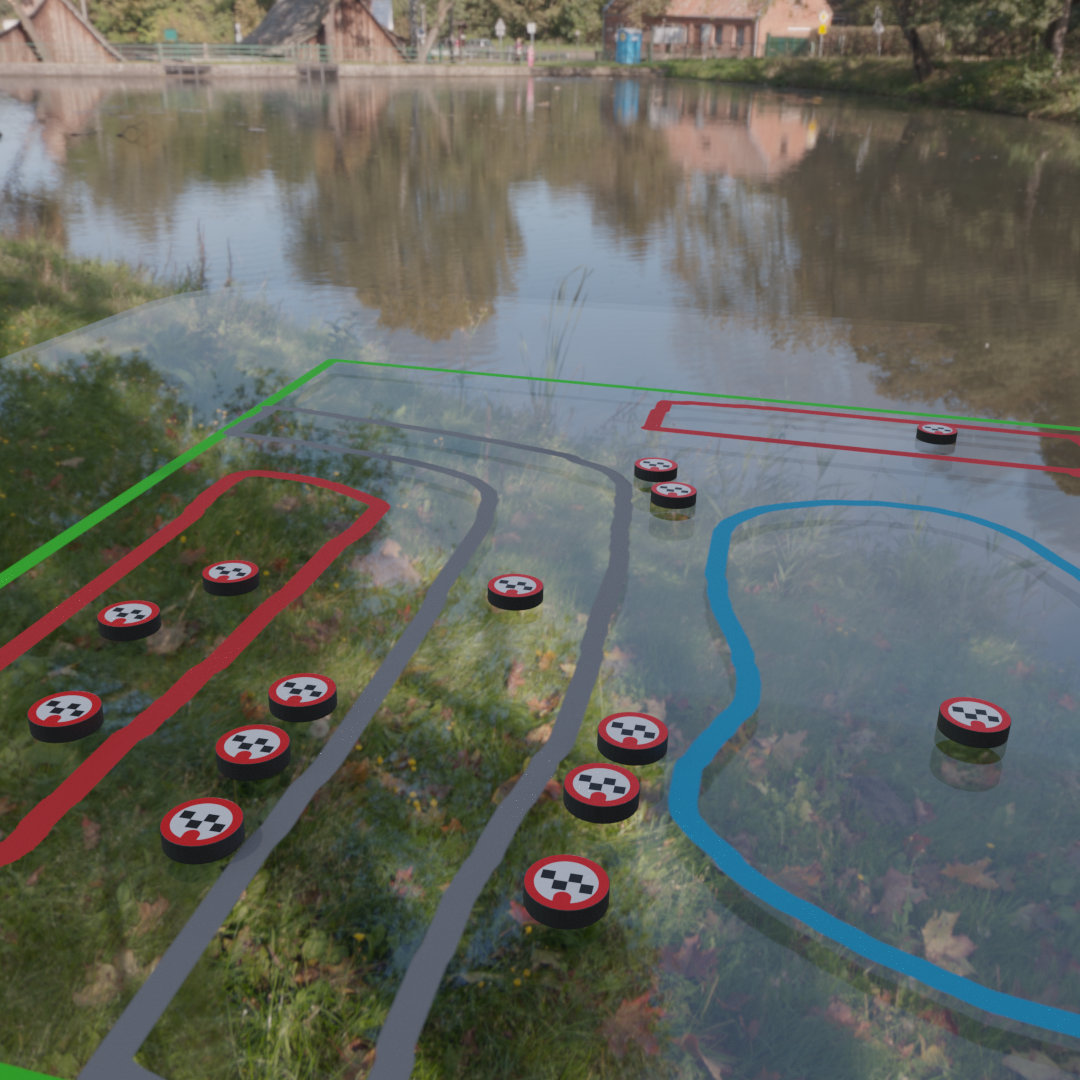
\includegraphics[width=1.0\linewidth]{figure/Evaluation/futuremarkers.png}
		\caption{Implementing this would allow architect to create flowerbeds, place multiple objects at a time, as well as change textures.}
		\label{fig:ftemarkers}
	\end{minipage}
	\hfill
	\begin{minipage}[b]{0.49\textwidth}
		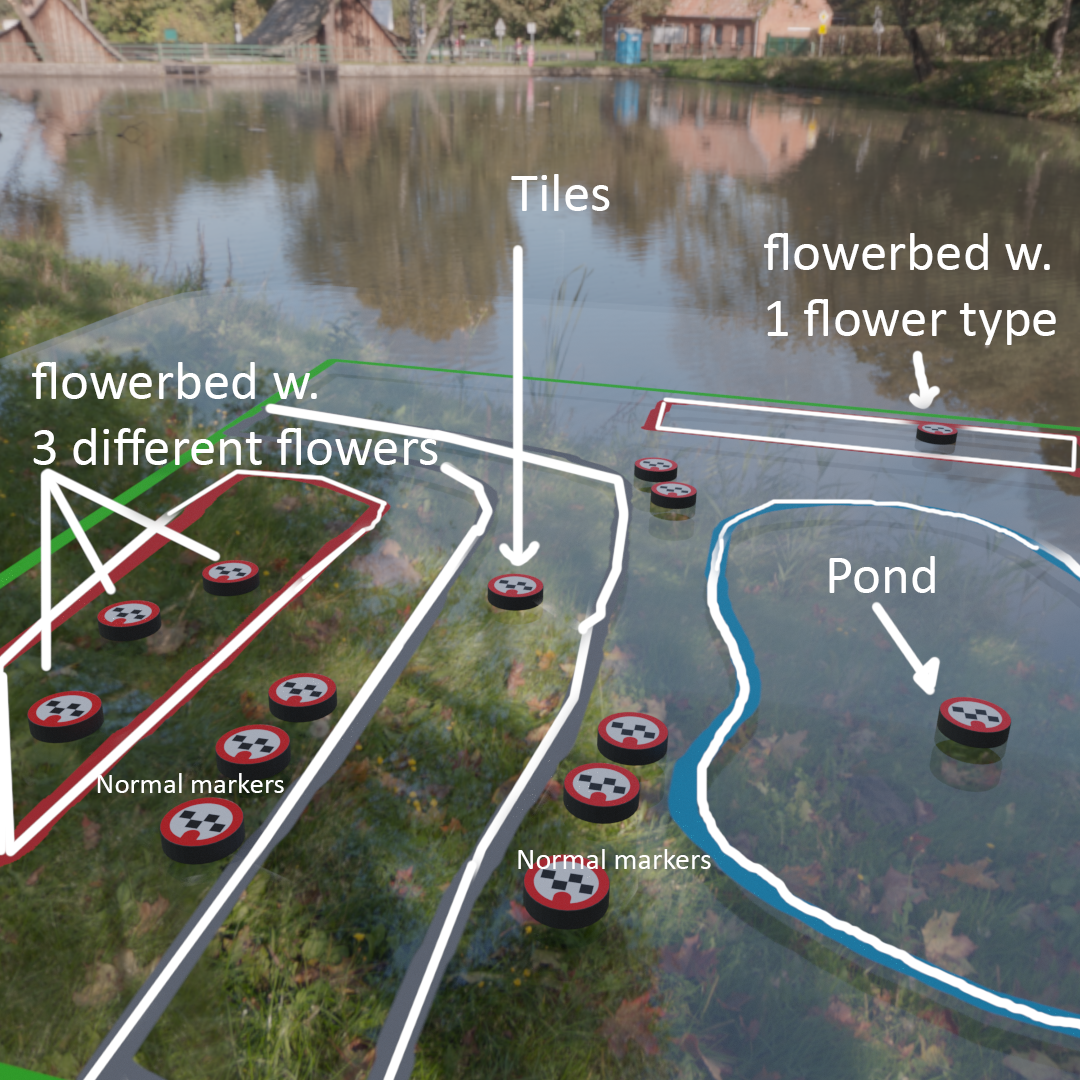
\includegraphics[width=1.0\linewidth]{figure/Evaluation/futuremarkerslegend.png}
		\caption{Explanation of what the Figure to the right would be interpreted as using this solution.}
		\label{fig:ftrmarkerslegend}
	\end{minipage}
\end{figure}
